\documentclass[a4paper,10pt]{article}
%\usepackage[latin1]{inputenc} % Paquetes de idioma
\usepackage[utf8]{inputenc} % Paquetes de idioma (Este encoding toma acentos :) )
\usepackage[spanish]{babel} % Paquetes de idioma
\usepackage{graphicx} % Paquete para ingresar gráficos
\usepackage{grffile}
\usepackage{hyperref}
\usepackage{fancybox}
\usepackage{amsmath}
\usepackage{amsfonts}
\usepackage{listings}
\usepackage{float}
% Paquetes de macros de Circuitos
%\usepackage{pstricks}
\usepackage{tikz}
% Encabezado y Pié de página
\usepackage{fancyhdr} % Paquete para encabezados y pie de página
\pagestyle{fancy} % Sin esta línea no se imprimiría el encabezado en todas las páginas

\fancyhf{} %  Borra el encabezado anterior (Por defecto escribe el títutlo de la sección en la que se encuentra la hoja
\setlength{\headheight}{22.55pt}
\fancyhead[L]{
	{\textsf{Facultad de Ingenier\'ia $-$ Universidad de Buenos Aires \\ 66.44 Instrumentos Electrónicos}}
}
%\addtocounter{page}{5}
\fancyhead[R]{\thepage}

\renewcommand{\footrulewidth}{0.4pt} % Ajusta el tamaño de las líneas separadoras en el pié de página
\renewcommand{\headrulewidth}{0.4pt} % Ajusta el tamaño de las líneas separadoras en el encabezado

\fancyfoot[L]{
	{\textsf{Trabajo Pr\'actico N$^{\circ}4$}: Mediciones de impedancias} \\
	{\textsf{Integrantes: Eduardo Sanchez, Francisco Soler}}
	}
		

% Carátula del Trabajo
\title{ \author{} % Lo pongo para que el warning no moleste :p
\setlength{\unitlength}{1cm} %  Especifica la unidad de trabajo
\thispagestyle{empty}

\begin{picture}(18,0)
\put(0,0){
\includegraphics[width=1.5cm, height=3cm]{Logo1.png}}

\put(10.5,0){
\includegraphics[width=3cm, height=3cm]{Logo2.png}}

\end{picture}
\\[1.5cm]
\begin{center}
	\textbf{{\Huge Facultad de Ingenier\'ia \\ Universidad de Buenos Aires}}\\[2cm]
	{66.44 Instrumentos Electrónicos}\\[0.5cm]
	{Trabajo Pr\'actico N$^{\circ}3$: Mediciones de impedancias}\\[2.5cm]
\end{center}

\begin{flushleft}
	\textbf{Integrantes:} \\[1cm]

	\begin{tabular}{|c|c|c|}
		\hline
		\textbf{\normalsize Padr\'on} & \textbf{\normalsize Nombre} & \textbf{\normalsize Email} \\
		\hline
		\normalsize 92903 & \normalsize Sanchez, Eduardo Hugo & \normalsize hugo\_044@hotmail.com \\
		\hline
		\normalsize 91227 & \normalsize Soler, Jos\'e Francisco & \normalsize francisco.\_tw@hotmail.com \\
		\hline
		\normalsize xxx & \normalsize Wawrynczak, Claudio  & \normalsize claudiozak@gmail.com \\
		\hline
	\end{tabular}
\end{flushleft}
\date{} % Hace que no se imprima la fecha en la cual se compilo el .tex
 }

\begin{document}
	\maketitle % Hace que el título anterior sea el principal del documento
	\newpage

	\tableofcontents % Esta línea genera un indice a partir de las secciones y 
					% subsecciones creadas en el documento
	\newpage
	

	\section{Objetivo}
	
	\indent	El objetivo del presente trabajo práctico es determinar el 
	comportamiento y fiabilidad de distintas funcionalidades del osciloscopio 
	tales como la FFT, el ruido tanto del oscoloscopio como de un generador, 
	y finalizando con las mediciones de velocidades de propagación utilizando 
	la reflectometría.
	
	\newpage
	\section{Desarrollo}

	\subsection{Medición 1 - Comportamiento FFT}
	\indent En esta medición se comparará el comportamiento de la funcionalidad
	FFT dispuesta en el osciloscopio utilizando cuatro tipos de ventanas 
	distintas, rectangular, hanning, hamming y blackman.\\
	\indent Se utilizarán 3 frecuencias contiguas de forma tal de observar como
	se modifica el pico de la sinc observada (Dependiendo del tipo de ventana, 
	queda recortado cuando no cae en un punto de medición de la FFT). \\
	\indent En las siguientes figuras, la frecuencia de la señal de la imagen de
	la izquierda corresponde a $11MHz$, la del medio a $11,7MHz$ y la de la 
	derecha a $11,9MHz$.\\
	\indent En la figura \ref{img001} se puede observar que efectivamente el 
	pico de la señal queda recortado. Logrando una diferencia de altura de la 
	señal en unos $1.5dB$.

	\begin{figure}[!htb]
		\centering
		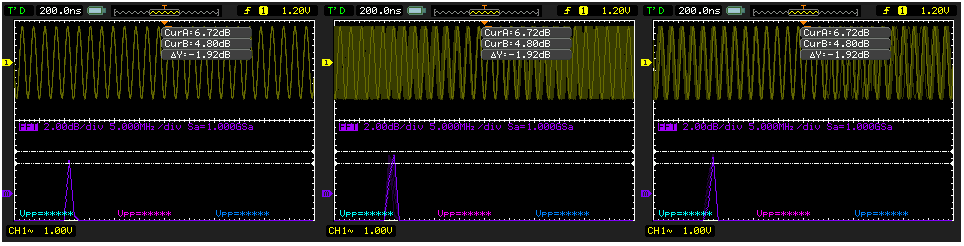
\includegraphics[width=8cm]
		{Imagenes/RectangularWindow.png}
		\caption{FFT de una señal senoidal utilizando una ventana Cuadrada.}
		\label{img001}
	\end{figure}

	\indent En la figura \ref{img002} se puede observar que , a diferencia
	de utilizar una ventana cuadrada, con la hanning el pico de la sinc no 
	disminuye en amplitud, por ende el pico siempre es el mismo.

	\begin{figure}[!htb]
		\centering
		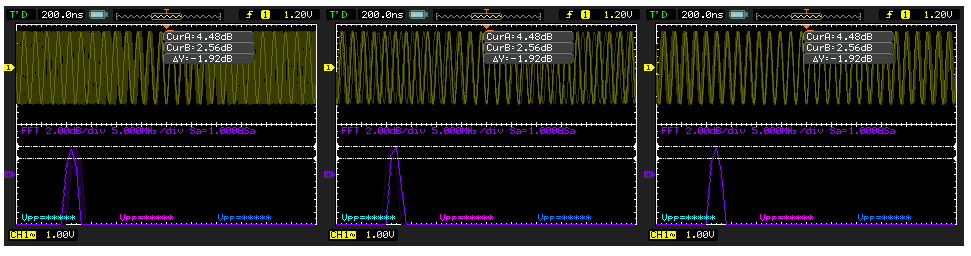
\includegraphics[width=8cm]
		{Imagenes/HanningWindow.png}
		\caption{FFT de una señal senoidal utilizando una ventana Hanning.}
		\label{img002}
	\end{figure}

	\indent En la figura \ref{img003} se puede observar que con la ventana 
	hamming no hay grandes diferencias con la hanning, simplemente se observa 
	un lóbulo levemente más angosto.

	\begin{figure}[!htb]
		\centering
		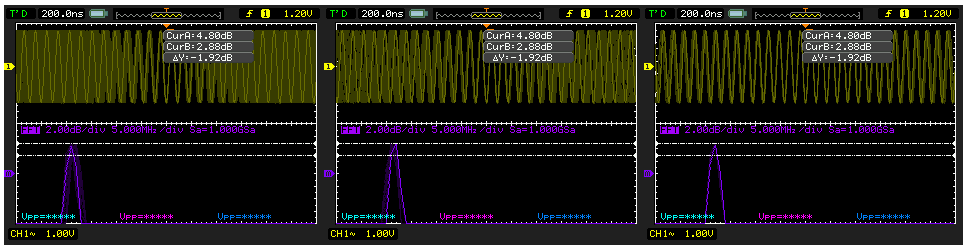
\includegraphics[width=8cm]
		{Imagenes/HammingWindow.png}
		\caption{FFT de una señal senoidal utilizando una ventana Hamming.}
		\label{img003}
	\end{figure}

	\indent En la figura \ref{img004} se puede observar que con la ventana 
	blackman no hay grandes diferencias con las dos anteriores, simplemente se 
	observa que el lóbulo es levemente más ancho y que el pico está en una 
	altura menor, aproximadamente en $2,90dB$ mientras que las otras están en 
	$4,80dB$.

	\begin{figure}[!htb]
		\centering
		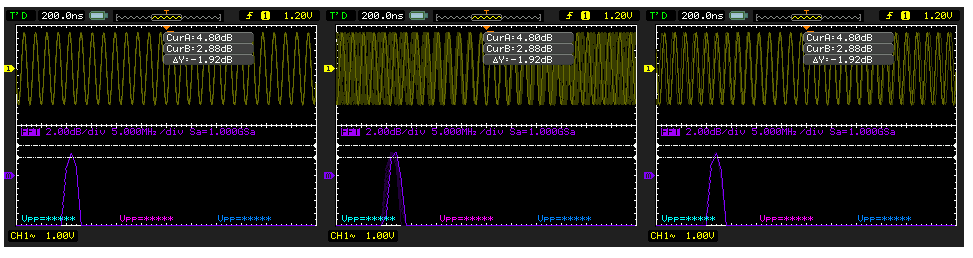
\includegraphics[width=8cm]
		{Imagenes/BlackmanWindow.png}
		\caption{FFT de una señal senoidal utilizando una ventana Blackman.}
		\label{img004}
	\end{figure}

	\subsection{Medición 2 - Ruido interno del osciloscopio}
	%\TODO
	\subsection{Medición 3 - Ruido de la fuente}
	%\TODO
	\subsection{Medición 4 - Tiempo de crecimiento de una compuerta}
	%\TODO
	\subsection{Medición 5 - Reflectometría}
	%\TODO
	\newpage 
	\section{Conclusión}
	%\TODO
\end{document}

